\documentclass{poly}
\usepackage{main}

\title{Arithmétique et Rationnels}
\date{}
\author{Seconde}

\begin{document}
\maketitle

\section{Arithmétique}
\subsection{Ensembles}
\begin{definition}
\hfill
\begin{itemize}
\item On note $\N$ l'ensemble des nombres entiers \textbf{Naturels} : il s'agit de tous les entiers plus grands ou égaux à $0$, comme $0$; $1$; $2$ \dots
\item On note $\Z$ l'ensemble des nombres entiers \textbf{relatifs} : il s'agit des entiers supérieurs, inférieurs ou égaux à \textbf{Zéro}, comme $-2$; $-1$; $0$; $1$; $2$ \dots
\end{itemize}
\end{definition}
\begin{definition}
\hfill

Pour dire qu'un nombre $n$ est un entier naturel, on écrit $n \in \N$. Cela se lit \emph{\og $n$ appartient à $\N$ \fg}.

Pour dire qu'un nombre $n$ est un entier relatif, on écrit $n \in \Z$. Cela se lit \emph{\og $n$ appartient à $\Z$ \fg}.
\end{definition}
\begin{example}
Vrai ou faux ? Répondre dans chacun des cas suivants.
\begin{alphaquestions}
\begin{minipage}{0.45\textwidth}
\item $6 \in \N$ 
\item $-9 \in \N$ 
\item $-4 \in \Z$ 
\end{minipage}
\hfill
\begin{minipage}{0.45\textwidth}
\item $12 \in \Z$         
\item $5 \notin \N$ 
\item $-8 \notin \N$ 
\end{minipage}
\end{alphaquestions}
\end{example}
\begin{proposition}
Tout nombre entier naturel est un nombre entier relatif. Du point de vue des ensembles, cette proposition se note $\N \subset \Z$.
\end{proposition}
\begin{example}
Placer les nombres suivants dans le schéma : $5$; $2$; $-10$; $0$ et $-6$.
\begin{center}
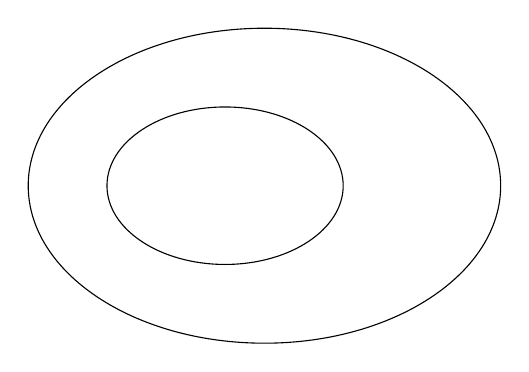
\begin{tikzpicture}
\draw (0,0) ellipse (3 and 2);
\draw (-0.5,0) ellipse (1.5 and 1);
\draw (2.5,0) node {$\Z$};
\draw (0.5,0) node {$\N$};
\end{tikzpicture}
\end{center}
\end{example}
\newpage
\subsection{Multiples et diviseurs}
\textbf{Nous travaillons avec les nombres de $\Z$. Dans ce contexte, on ne considère pas les divisions réelles, ni les fractions.}
\begin{definition}
Soit $a$ et $b$ deux entiers relatifs.
\begin{itemize}
\item $a$ est un \textbf{multiple} de $b$ si et seulement si il existe $k \in \Z$ tel que $a = k \times b$.
\item $b$ est un \textbf{diviseur} de $a$ si et seulement si il existe $k \in \Z$ tel que $a = k \times b$.
\end{itemize}
\end{definition}
\begin{example}
\hfill
\begin{itemize}
\item Le nombre $10$ est un multiple de $2$ : en effet, il existe un nombre entier relatif $k = 5$ tel que $10 = k \times 2$.
\item Le nombre $7$ est un diviseur de $-28$ : en effet, il existe un nombre entier relatif $k = -4$ tel que $28 = k \times 7$.
\end{itemize}
\end{example}
\begin{example}
\hfill

Le nombre $36$ est-il un multiple de $3$ ? Justifier. 

Le nombre $-8$ est-il un diviseur de $128$ ? Justifier. 
\end{example}

\begin{remark}
$0$ est divisible par n'importe quel nombre. Ou, de façon équivalente, $0$ est le multiple de n'importe quel nombre. 
\end{remark}

\begin{proposition}
La somme de deux multiples de $a$ est un multiple de $a$.
\end{proposition}
\begin{proof} \textbf{Démonstration dans le cahier.}

\end{proof}
\begin{definition}
\hfill
\begin{itemize}
\item Un nombre entier relatif est \textbf{pair} si et seulement s'il est divisible par $2$.
\item Un nombre entier relatif est \textbf{impair} si et seulement s'il n'est pas pair. 
\end{itemize}
\end{definition}
\begin{example}
\hfill

Le nombre $12$ est pair : en effet, il est divisible par $2$, car $12 = 2 \times 6$.

Le nombre $-27$ est impair : en effet, il n'est pas pair, car il n'existe pas d'entier relatif $k$ vérifiant $-27 = 2 \times k$.
\end{example}

\begin{proposition}
Un nombre $n \in \Z$ est impair si et seulement si il existe $p \in \Z$ tel que $n = 2 \times p + 1$.
\end{proposition}

\begin{proposition}
Soit $x$ et $y$ deux entiers relatifs. Alors, les tableaux suivants décrivent la parité de $x + y$ et de $x \times y$.
\vspace*{0.5cm}

\begin{minipage}{0.30\textwidth}
\begin{tabular}{|c|c|c|}
\hline
$x + y$&$y$ pair&$y$ impair\\
\hline
$x$ pair&pair& impair\\
\hline
$x$ impair& impair& pair\\
\hline
\end{tabular}    
\end{minipage}
\hfill
\begin{minipage}{0.30\textwidth}
\begin{tabular}{|c|c|c|}
\hline
$x \times y$&$y$ pair&$y$ impair\\
\hline
$x$ pair&pair& pair\\
\hline
$x$ impair& pair& impair\\
\hline
\end{tabular}    
\end{minipage}
\hfill
\begin{minipage}{0.30\textwidth}
\begin{tabular}{|c|c|c|}
\hline
$x^2$&$x$ pair&$x$ impair\\
\hline
&pair& impair\\
\hline
\end{tabular}    
\end{minipage}
\end{proposition}
\begin{proof}
On démontre dans le cahier uniquement la propriété suivante : si $x$ est un entier relatif impair, alors $x^2$ est impair.
\end{proof}

\newpage
\subsection{Nombres premiers}
\begin{definition}
Un nombre entier naturel $n \in \N$ est \textbf{premier} si et seulement si il admet exactement deux diviseurs positifs : $1$ et lui-même. 
\end{definition}
\begin{remark}
\hfill
\begin{itemize}
\item Traditionnellement, un nombre premier est \textbf{positif} : on ne s'intéresse qu'aux entiers naturels dans ce cadre.
\item Le nombre $1$ n'est \textbf{\textsc{pas}} premier : il n'admet qu'un seul diviseur positif. 
\end{itemize}
\end{remark}
\begin{example}
Les nombres suivants sont premiers: $2; 3; 5; 7; 11; 13; 17; 19 \dots$
\end{example}
\begin{theorem}
Tout entier naturel supérieur ou égal à $2$ peut s'écrire comme un produit de nombres premiers. Écrite dans l'ordre croissant des facteurs, \textbf{cette décomposition est unique}
\end{theorem}
\begin{example}
\hfill
\begin{itemize}
\item $18 = 2 \times 3 \times 3$
\item $68 =$  
\item $132 =$ 
\item $85 =$ 
\end{itemize}
\end{example}
\begin{example}
On peut écrire des fractions sous forme irréductible à l'aide de la décomposition du numérateur et du dénominateur en produit de facteurs premiers.
\begin{itemize}
\item $\dfrac{500}{75} = \dfrac{2 \times 2 \times 5 \times \cancel{5} \times \cancel{5}}{3 \times \cancel{5} \times \cancel{5}} = \dfrac{2 \times 2 \times 5}{3} = \dfrac{20}{3}$
\item $\dfrac{126}{24} =$ 
\item $\dfrac{3}{45} =$ 
\end{itemize}
\end{example}
\begin{proposition}
Soit $n \in \N$. Alors $n$ est premier si et seulement s'il n'existe aucun diviseur premier de $n$ entre $2$ et $\sqrt{n}$ 
\end{proposition}
\begin{exercize}
\hfill
\begin{alphaquestions}
\item Montrer que $503$ est premier.
\item Montrer que $323$ n'est pas premier.
\end{alphaquestions}
\end{exercize}

\newpage
\section{Nombres rationnels}
\subsection{Ensembles}
\begin{definition}
\hfill
\begin{itemize}
\item On note $\D$ l'ensemble des \textbf{nombres décimaux}, c'est-à-dire l'ensemble des nombres dont l'écriture décimale est finie (nombre fini de chiffres après la virgule).
\item On note $\Q$ l'ensemble des \textbf{nombres rationnels}, c'est-à-dire l'ensemble des nombres pouvant s'écrire sous la forme d'une fraction d'entiers
\begin{equation*}
\dfrac{a}{b}
\end{equation*}
avec $a \in \Z$, $b \in \N$ et $n \neq 0$.
\end{itemize}
\end{definition}
\begin{example}
Les nombres suivants sont des nombres décimaux : $1,23$; $2$; $-3,4$ \dots

Les nombres suivants sont des nombres rationnels :
$1,23$; $\dfrac{4}{2}$; $\dfrac{1}{3}$ \dots
\end{example}
\begin{proposition}
Tout nombre $x \in \D$ est de la forme
\begin{equation*}
x = \dfrac{a}{10^k}
\end{equation*}
tel que $a \in Z$ et $k \in \N$.
\end{proposition}
\begin{remark}
\hfill
\begin{itemize}
\item Cette proposition nous permet d'affirmer que tout nombre décimal est un nombre rationnel. Cela s'écrit $\D \subseteq \Q$.
\item Tout entier relatif est un nombre décimal. On en déduit que tout entier relatif est un nombre rationnel. En effet, si $x \in \Z$, alors $x = \dfrac{x}{1} = \dfrac{x}{10^0}$. 
\end{itemize}
\end{remark}
\begin{example}
Compléter le schéma suivant en mettant chaque nombre dans l'ensemble le plus petit le contenant :
$2$; $-4,3$; $\dfrac{1}{7}$; $\dfrac{-10}{2}$; $21,333\dots$; $0$; $\dfrac{10}{25}$.
\begin{center}
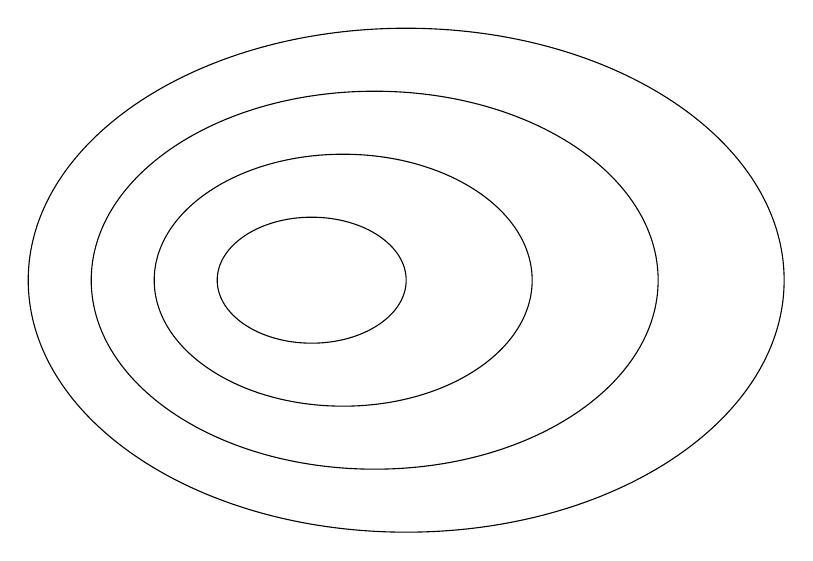
\begin{tikzpicture}[scale=0.8]
\draw (1,0) ellipse (6 and 4);
\draw (0.5,0) ellipse (4.5 and 3);
\draw (0,0) ellipse (3 and 2);
\draw (-0.5,0) ellipse (1.5 and 1);
\draw (6.5,0) node {$\Q$};
\draw (4.5,0) node {$\D$};
\draw (2.5,0) node {$\Z$};
\draw (0.5,0) node {$\N$};
\end{tikzpicture}    
\end{center}
\end{example}
\newpage
\subsection{Reconnaitre un nombre décimal ou rationnel}
\subsubsection{Fractions}
\begin{definition}
Une fraction $\dfrac{a}{b}$ est dite \textbf{irréductible} si et seulement si le seul diviseur commun à $a$ et $b$ est $1$. 
\end{definition}
\begin{example}
\hfill
\begin{alphaquestions}
\item La fraction $\dfrac{67}{15}$ est-elle irréductible ? 
\item La fraction $\dfrac{789}{456}$ est-elle irréductible ? 
\end{alphaquestions}
\end{example}
\begin{proposition}
Soit une fraction $\dfrac{a}{b}$ \textbf{sous forme irréductible}. Si la décomposition en facteurs premier de $b$ ne fait apparaître uniquement des $2$ et des $5$, alors $x$ est un nombre décimal.
\end{proposition}
\begin{example}
\hfill
\begin{alphaquestions}
\item $\dfrac{3}{50}$ est-il décimal ? 
\item $\dfrac{8}{12}$ est-il décimal ? 
\item $\dfrac{45}{12}$ est-il décimal ? 
\end{alphaquestions}
\end{example}
\subsubsection{Écriture décimale}
\begin{remark}
Si le développement décimal d'un nombre $x$ est \textbf{périodique}, alors ce nombre est rationnel.
\end{remark}
\begin{example}
\hfill
\begin{itemize}
\item $0,12121212...$ est rationnel, la période $12$ se répète indéfiniment.
\item $115,0123456789...$ n'est pas rationnel (a priori), on ne détecte pas de période.
\item $-76,89001001001001...$ est rationnel, la période $100$ se répète indéfiniment.
\end{itemize}
\end{example}
\section{Démonstrations}

\begin{proposition}
$\dfrac{1}{3}$ n'est pas décimal.
\end{proposition}

\begin{theorem}
Le nombre $\sqrt{2}$ n'est pas rationnel.
\end{theorem}
\begin{proof}
Voir cahier. \textbf{À savoir refaire}.
\end{proof}



\end{document}

